\documentclass[,a4paper,12pt,french]{article}

\usepackage[TD]{../../../Style}

\pagestyle{empty}

% Début du document
%%%%%%%%%%%%%%%%%%%
\begin{document}

\titre{Variations de fonctions}

\begin{multicols*}{2}

\begin{exercice}
Soit $f$ une fonction définie sur $[-5;5]$.
\begin{enumerate}
\item Comparer $f(-1)$ et $f(1)$ en sachant que $f$ est croissante.
\item Comparer $f(3)$ et $f(0)$ en sachant que $f$ est décroissante.
\end{enumerate}
\end{exercice}

\begin{exercice}
On a représenté une fonction $f$ ci-dessous. Vrai ou faux?
\begin{center}
\begin{tikzpicture}[scale=\echellepgf]
\begin{axis}[
styleglobal,
width=0.8*\echellepgfinv*\linewidth,
xmin=-3.5, xmax= 5.5,
ymin=-1.5, ymax=3.5,
xtick distance=1,
ytick distance=1,
minor x tick num=1,
minor y tick num=1,
]
\addplot[styleplot,domain=(-3:5)] plot {0.25*(x-1)^2-1} node[pos=0.85,below right] {$\mathscr C_f$} \pointsextremites;
\end{axis}
\end{tikzpicture}
\end{center}
\begin{enumerate}
\item $f$ est croissante sur $[1;5]$
\item $f$ est décroissante sur $[-2;3]$
\item $f$ est décroissante sur $[-3;-2]$.
\end{enumerate}
\end{exercice}

\begin{exercice}
Soit $g$ une fonction définie sur l'intervalle $[0;4]$ et telle que:
\begin{itemize}
\item $f$ est croissante sur l'intervalle $[0;2]$
\item $f$ est décroissante sur l'intervalle $[2;4]$
\item $f(0)=f(4)=5$ et $f(2)=10$
\end{itemize}
Dresser le tableau de variations de $g$ sur $[0;4]$.
\end{exercice}

\begin{exercice} \label{schemafonctions}
Dresser le tableau de variation des fonctions $f$, $g$ et $h$ définies sur le repère suivant:
\begin{center}
\begin{tikzpicture}[scale=\echellepgf]
\begin{axis}[
styleglobal,
width=0.8*\echellepgfinv*\linewidth,
xmin=-0.5, xmax= 8.5,
ymin=-2.5, ymax=3.5,
xtick distance=1,
ytick distance=1,
minor x tick num=1,
minor y tick num=1,
]
\addplot[styleplot,domain=(0:8)] plot {0.5*x-1.5)} node[pos=0.75,above] {$\mathscr C_f$} \pointsextremites;
\addplot[styleplot,color=DarkRed,densely dashed] plot coordinates{(0,-2) (1,-1) (2,2) (3,3) (5,1) (6,0) (8,-1.5)} node[pos=0.5,above right] {$\mathscr C_g$} \pointsextremites;
\addplot[styleplot,densely dotted,color=DarkGreen] plot coordinates{(0,3) (2,2) (3,0) (4,-2) (6,0) (7,2) (8,3)} node[pos=0.07,above right] {$\mathscr C_h$} \pointsextremites;
\end{axis}
\end{tikzpicture}
\end{center}
\end{exercice}

\begin{exercice} \label{exoTabVar}
Tracer la représentation graphique d'une fonction $f$ définie sur $[-3;5]$ dont le tableau de variations est donné ci-dessous:

\begin{center}
\begin{tikzpicture}
\tkzTabInit[lgt=1.4,espcl=1.7]{$x$/1, $f(x)$/1.7}{$-3$,$-2$,1,4,5}
\tkzTabVar{+/5, -/3, +/4, -/1, +/4 }
\end{tikzpicture}
\end{center}
\end{exercice}

\begin{exercice}
Voici les courbes représentatives dans un repère de deux fonctions $f$ et $g$ dont on donne les tableaux de variations. Associer chaque fonction à la courbe $\mathscr C_1$ ou $\mathscr C_2$ qui la représente.
\begin{center}
\begin{tikzpicture}[scale=\echellepgf]
\begin{axis}[
styleglobal,
width=0.8*\echellepgfinv*\linewidth,
xmin=-4.5, xmax=7.5,
ymin=-2.5, ymax=4.5,
xtick distance=1,
ytick distance=1,
minor x tick num=1,
minor y tick num=1,
]
%\addplot[styleplot,tension=0.25] plot coordinates {(-4,1) (-1,-2) (3,4) (7,1)} node[pos=0.75,above right] {$\mathscr C_2$} \pointsextremites;
%\addplot[styleplot,tension=0.25,color=blue,densely dashed] plot coordinates {(-4,1) (-2,-1) (4,3) (7,1)} node[pos=0.75,below] {$\mathscr C_1$} \pointsextremites;
%Bezier: A gauche: points de passage, à droite: points de contrôle pour la direction
\draw[line width=1.3pt] (-4,1) .. controls  (-3.5,0) and (-1.75,-2)
					 .. (-1,-2) node[pos=0,stylepointextremites] {} .. controls (0.25,-2) and (1.5,4) 
					 .. (3,4) .. controls (4,4) and (6,2.5) 
					 .. (7,1) node[pos=0.3,above right] {$\mathscr C_1$} node[pos=1,stylepointextremites] {};
\draw[line width=1.3pt,color=blue,densely dashed]
						(-4,1) .. controls  (-3.5,0) and (-2.75,-1)
					 .. (-2,-1) .. controls (-0.75,-1) and (2.5,3) 
					 .. (4,3)   .. controls (5,3) and (6,2.5) 
					 .. (7,1) node[pos=0.1,below] {$\mathscr C_2$};
\end{axis}
\end{tikzpicture}

\begin{tikzpicture}
\tkzTabInit[lgt=1.4,espcl=1.7]{$x$/1, $f(x)$/1.7}{$-4$,$-2$,3,7}
\tkzTabVar{+/1, -/$-1$, +/4, -/1 }
\end{tikzpicture}

\begin{tikzpicture}
\tkzTabInit[lgt=1.4,espcl=1.7]{$x$/1, $g(x)$/1.7}{$-4$,$-1$,4,7}
\tkzTabVar{+/1, -/$-2$, +/3, -/1 }
\end{tikzpicture}
\end{center}
\end{exercice}

\begin{exercice}
On se donne les fonctions $f$ et $g$, représentées sur le repère suivant:
\begin{center}
\begin{tikzpicture}[scale=\echellepgf]
\begin{axis}[
styleglobal,
width=0.8*\echellepgfinv*\linewidth,
xmin=-2.5, xmax= 8.5,
ymin=-2.5, ymax=3.5,
xtick distance=1,
ytick distance=1,
minor x tick num=1,
minor y tick num=1,
]
\addplot[styleplot,tension=0.3] plot coordinates{(-2,-1.5) (-0.5,1) (2,1.5) (3,3) (5,1) (6,2) (8,-2)} node[pos=0.72,above] {$\mathscr C_f$} \pointsextremites;
\addplot[styleplot,densely dashed,color=blue] plot coordinates{(-2,3) (0,1) (3,-1.5) (4,1) (5,-1.5) (7,2) (8,2.5)} node[pos=0.98,below] {$\mathscr C_g$} \pointsextremites;
\end{axis}
\end{tikzpicture}
\end{center}
\begin{enumerate}
\item Donner le maximum de $f$ et le(ou les) antécédents associés.
\item Donner le minimum de $g$ et le(ou les) antécédents associés.
\item Donner le maximum de $g$ sur l'intervalle $[1;6]$.
\end{enumerate}
\end{exercice}

\begin{exercice}
On se donne la fonction $f$ définie dans l'exercice \ref{exoTabVar}.
\begin{enumerate}
\item Donner le maximum de $f$ sur $[-3;5]$ et le(ou les) antécédents associés.
\item Donner le minimum de $f$ sur $[-3;5]$ et le(ou les) antécédents associés.
\item Donner le minimum de $f$ sur l'intervalle $[-2,5;3]$.
\end{enumerate}
\end{exercice}

\end{multicols*}

\newpage \

\vfill

\begin{center}
\begin{tikzpicture}[scale=\echellepgf]
\begin{axis}[
styleglobal,
labelgros,
width=0.4*\echellepgfinv*\linewidth,
xmin=-3.5, xmax= 6.5,
ymin=-0.5, ymax=5.5,
xtick distance=1,
ytick distance=1,
minor x tick num=1,
minor y tick num=1,
]
\end{axis}
\end{tikzpicture}
\end{center}

\vfill

\end{document}
